\documentclass[notes=hide,hyperref={dvipdfmx,pdfpagelabels=false}]{beamer}
\title{Einführung in Sage - Einheit 1}
\subtitle{Organisatorisches, Was ist Sage?, Streifzug durch Sage}
\mode<article>
{
  \usepackage{fullpage}
  \usepackage{pgf}
  \usepackage[xetex]{hyperref}
  \setjobnamebeamerversion{beamer}
}

\mode<presentation>
{
  %\usetheme{Frankfurt}
 %\usetheme{My}
  \usetheme{Madrid}
  % or ...
%\usecolortheme{seagull}
  %\setbeamercovered{transparent}
  %\setbeamercovered{dynamic}
  % or whatever (possibly just delete it)
}
\usenavigationsymbolstemplate{}
\usefonttheme{structurebold}
\usepackage{multimedia}
%\usepackage{tikz}
\usepackage{fontspec,xunicode,xltxtra}

%\usepackage{polyglossia}
%\setdefaultlanguage[spelling=new, latesthyphen=true]{german}
%\setsansfont{DejaVu Sans}
%\setsansfont{Verdana}
%\setsansfont{Arial}
%\setromanfont{Linux Libertine O}
%\setsansfont{Linux Biolinum O}

\setbeamertemplate{footline}
{
\leavevmode
%\hbox{\begin{beamercolorbox}[wd=.5\paperwidth,ht=2.5ex,dp=1.125ex,
%leftskip=.3cm plus1fill,rightskip=.3cm]{author in head/foot}%
%    \usebeamerfont{author in head/foot}\insertshortauthor
%  \end{beamercolorbox}%
%  \begin{beamercolorbox}[wd=.5\paperwidth,ht=2.5ex,dp=1.125ex,leftskip=.3cm,
%rightskip=.3cm plus1fil]{title in head/foot}%
%    \usebeamerfont{title in head/foot}\insertshorttitle\hfill

\hfill\insertframenumber  \hspace{3pt}

%\inserttotalframenumber
%\hspace*{2ex}
%  \end{beamercolorbox}}%
  \vskip3pt%
}

\usepackage[ngerman]{babel}
\selectlanguage{ngerman}

%
% math/symbols
%
\usepackage{amssymb}
\usepackage{amsthm}
% \usepackage{latexsym}
\usepackage{amsmath}
%\usepackage{amsxtra} %Weitere Extrasymbole
%\usepackage{empheq} %Gleichungen hervorheben
%\usepackage{bm}
 %\bm{A} Boldface im Mathemodus

\usepackage{cellspace}
\setlength{\cellspacetoplimit}{2pt}
\setlength{\cellspacebottomlimit}{2pt}

%%%%%%%%%%%%%%%%%% Fuer Frames [fragile]-Option verwenden!
%Programm-Listing
%%%%%%%%%%%%%%%%%%
%Listingsumgebung fuer verbatim
%Grauhinterlegeter Text
%Automatischer Zeilenumbruch ist aktiviert
\usepackage{listings}
\definecolor{lgray}{gray}{0.80}
%\lstset{backgroundcolor=\color{lgray}, frame=single, basicstyle=\ttfamily, breaklines=true}
\lstnewenvironment{sage}{\lstset{backgroundcolor=\color{lgray},language=Python, emphstyle=\color{red}, frame=single, basicstyle=\ttfamily, breaklines=true,mathescape =true,escapechar=§}}{}


\usepackage{mydef}
%\usepackage{cmap} % you can search in the pdf for umlauts and ligatures
\usepackage{colonequals} %corrects the definition-symbols \colonequals (besides others)
\title{Einführung in Sage}
%
%\subtitle{Disputation} % (optional)

\author{Jochen Schulz}
% - Use the \inst{?} command only if the authors have different
%   affiliation.

\institute{Georg-August Universit\"at G\"ottingen \pgfimage[height=0.5cm]{../figures/unilogo3}}
% - Use the \inst command only if there are several affiliations.
% - Keep it simple, no one is interested in your street address.

\date{\today}

\subject{Sage}
% This is only inserted into the PDF information catalog. Can be left
% out. 

% If you have a file called "university-logo-filename.xxx", where xxx
% is a graphic format that can be processed by latex or pdflatex,
% resp., then you can add a logo as follows:

%\logo{\pgfimage[height=0.5cm]{figures/unilogo3}}


% Delete this, if you do not want the table of contents to pop up at
% the beginning of each subsection:

\AtBeginSection[]
{
  \begin{frame}<beamer>
    \frametitle{Aufbau}
    \tableofcontents[currentsection,currentsubsection]
  \end{frame}
}

\AtBeginSubsection[]
{
  \begin{frame}<beamer>
    \frametitle{Aufbau}
    \tableofcontents[currentsection,currentsubsection]
  \end{frame}
}



%%%%%%%%%%%%%%%%%%%
%Neue Definitionen
%%%%%%%%%%%%%%%%%%%

%Newcommands
\newcommand{\Fun}[1]{\mathcal{#1}}      %Mathcal fuer Funktoren
\newcommand{\field}[1]{\mathbb{#1}}     %Grundkoerper ?? in mathds

\newcommand{\A}{\field{A}}              %Affines A
\newcommand{\C}{\field{C}}              %Complexes C
\newcommand{\Fp}{\field{F}_{\!p}}       %Endlicher Koerper mit p Elementen
\newcommand{\Fq}{\field{F}_{\!q}}       %Endlicher Koerper mit q Elementen
\newcommand{\Ga}{\field{G}_{a}}         %Add Gruppenschema
\newcommand{\K}{\field{K}}              %Generischer Koerper 
\newcommand{\N}{\field{N}}              %Nat Zahlen
\newcommand{\Pj}{\field{P}}             %Projektives P
\newcommand{\R}{\field{R}} 		%Reelle Zahlen
\newcommand{\Q}{\field{Q}}              %Rationale Zahlen  
\newcommand{\Qt}{\field{H}}             %Quaternionen 
\newcommand{\V}{\field{V}}              %Vektorbuendel V
\newcommand{\Z}{\field{Z}}              %Ganze Zahlen

\newcommand{\fdg}{\;|\;}                 %fuer die gilt

%Operatoren
\DeclareMathOperator{\Abb}{Abb}
%\usepackage{sagetex}

\begin{document}
\lstset{basicstyle={\lstbasicfont\footnotesize}}


\maketitle

%%%%%%%%%%%%%%%%%%%%%%%%%%%%%%%%%%%%%%
\section*{Organisatorisches}
%%%%%%%%%%%%%%%%%%%%%%%%%%%%%%%%%%%%%

\begin{frame}{Organisatorisches}
\begin{itemize}
\item Anmeldung über StudIP \\
      \url{https://www.studip.uni-goettingen.de/}

{\color{blue}{Einführung in Sage (Mathematische Anwendersysteme) (WS 2011/2012)}}
\item Aufgabenblätter und  Vorlesungsworksheets sind unter \url{https://sage.math.uni-goettingen.de} zu erhalten.
\item Vorlesungsfolien, Musterlösungen und Zusammenfassungen können aus StudIP heruntergeladen werden. 
\pause
\begin{block}{Dozent}
Jochen Schulz\\
NAM, Zimmer 04 (Erdgescho{\ss})\\
Telefon: 39-4525
Email: \href{mailto:schulz@math.uni-goettingen.de}{\texttt{schulz@math.uni-goettingen.de}}\\
XMPP: \url{schulz@jabber.num.math.uni-goettingen.de}\\

\end{block}
\end{itemize}
\end{frame}

\begin{frame}{Starten des Programms}
\textbf{Vor.:} Account im CIP-Pool der Mathematischen Fakultät (MI und NAM): Registrierungs-Formular unter \url{https://ldap.math.uni-goettingen.de} (\alert{Stud.It-Account} nötig!)\\
\textbf{Intranet/Wiki} (\url{https://wiki.math.uni-goettingen.de})
\begin{itemize}
\item Sage ist in Version 4.7.2 installiert
\item Nutzen von Sage: 
\begin{itemize}
\item Über \url{https://sage.math.uni-goettingen.de}. Login mit Studentendaten.
\item im Menu unter Education: \texttt{sagenotebook} startet (lokale) gui.\\
\item im Terminal: \texttt{sage}
\item Remote per \alert{nxclient} oder \alert{x2goclient}
auf \texttt{login.math.uni-goettingen.de} und \texttt{sc1.math.uni-goettingen.de} bis 
\texttt{sc8.math.uni-goettingen.de}
\end{itemize}
\end{itemize}
\end{frame}

\begin{frame}{Ablauf der Veranstaltung}
\begin{itemize}
\item Blockveranstaltung vom  20.2-2.3.2012
\item \alert{Vorlesung:} 9 Uhr bis 11 Uhr
\item \alert{Übungsbetrieb}: 4 Gruppen \`a je 1h 15min (Besprechung Aufgaben u. Praktikum, Teilnahme freiwillig)
\begin{itemize}
\item 11:00-12:15 	
\item 12:15-13:15 Mittagspause
\item 13:15-14:30 
\item 14:30-15:45
\item 15:45-17:00 
\end{itemize}
\item \alert{Praktikum:} von 11:00 bis 19:00 Uhr Computerräume im Keller des MI.
\item \alert{Übungsbetrieb:}
\begin{itemize}
\item 1 Übungszettel/Tag.
\item Klausurzulassung: 3 beliebige markierte Aufgaben/Woche testieren lassen. 
\item Alternativ: Projektarbeit durchführen (Projekte im StudIP zu finden)
\end{itemize}
\item \alert{Klausur 1:} 9.3.2012; 10:00 - 11:30; HS1/Maximum.
\item \alert{Klausur 2:} 23.3.2012; 10:00 - 11:30; HS1.
\end{itemize}
\end{frame}

\begin{frame}{Inhalt der Vorlesung}
\alert{Ziel:} Wiederholung des Stoffs Diff 1 und AGLA 1 mittels der Methoden der Computeralgebra und der numerischen Rechnung.
\begin{description}
 \item[1. Tag]Organisatorisches, Aufbau von Sage, Streifzug durch Sage
\item [2. Tag] Grundlagen, Symbolisches Rechnen, Gleichungen
\item [3. Tag] Mengen, Zahlen
\item [4. Tag] Matrizen, Vektorräume, Funktionen
\item [5. Tag] Datencontainer, Lineare Abbildungen, Eigenwert und Eigenvektoren
\item [6. Tag] Folgen, Reihen, Potenzreihen, Vertiefung Schleifen
\item [7. Tag] Funktionen, Grenzwerte, Funktionenfolgen, Grafiken
\item [8. Tag] Differentation, Taylorsche Formel, Integration
\item [9. Tag] Strings, interaktive Grafiken, GeoGebra, Komplexe Beispiele
\item [10. Tag] Fragestunde
\end{description}
\end{frame}

\begin{frame}{Aufbau}
\tableofcontents
\end{frame}



%%%%%%%%%%%%%%%%%%%%%%%%%%%%%%
\section{Was ist Sage?}
%%%%%%%%%%%%%%%%%%%%%%%%%%%%%%%%%

\begin{frame}{Mathematik-Software}

\begin{block}{Computeralgebra (CAS)}
\alert{exakte} Berechnungen von mathematischen Objekten
\end{block}
\bigskip

\begin{block}{Mathematische Objekte} 
Natürliche Zahlen, reelle Zahlen, Polynome, Funktionen,
Gruppen, Ringe, \ldots
\end{block}

\begin{block}{Numerischen Berechnungen}
\alert{näherungsweise} Berechnung von mathematischen Objekten. Im Computer 
{\color{blue}Gleitpunktdarstellung} genannt.
\end{block}


\begin{block}{Computeralgebra != Numerische Berechnung}
\begin{tabular}{ll}
 Mathematische Objekte & $\pi$, $\sqrt{2}$\\
 Gleitpunktdarstellung (8 Stellen)& $3.1415927$, $1.4142136$
\end{tabular}
\end{block}
\end{frame}

\begin{frame}{Mathematik-Software (Auswahl)}
\begin{small}
\begin{block}{}
\begin{tabular}{ll}
\alert{Sage} & Mathematik-Software; Symbolisch und numerisch (GPL)\\
 \alert{Maxima} & GPL, von Sage benutzt\\
\alert{Mathematica} &einer der Grossen CAS (kommerziell)\\
 \alert{Maple} &einer der Grossen CAS (kommerziell)\\
\alert{Matlab} &Für numerische Rechnungen (inkl. Mupad,kommerziell)\\
\alert{Octave} &Für numerische Rechnungen (GPL)\\
\alert{Magma} & Algebra, Zahlentheorie, Geometrie (kommerziell)\\
 \alert{SymPy} &Phython-Bibliotheken; als CAS-Verwendbar (GPL)\\
 \alert{SymbolicC++} &Bibliotheken zur CA in C++ (GPL)
\end{tabular}

\medskip
Überblick:\\{\scriptsize
\url{http://en.wikipedia.org/wiki/Mathematical_software} }
\end{block}

%\alert{Spezialanwendungen}: & Cadabra (Körpertheorie)\\
%& PARI/GP (Zahlentheorie, Teil von Sage)\\
%& GAP (Gruppentheorie, Teil von Sage) \\
%& Macaulay (Algebraische Geometrie)\\
%& Singular (Algebraische Geometrie, Teil von Sage)
%\end{tabular}
\end{small}
\end{frame}

\begin{frame}{Sage}
\begin{itemize}
\item Ein Open-source (GPL) Mathematik Software System
\item Verfügbar seit 24 Februar 2005
\item Alternative zu den 4 M's: Magma, Maple, Mathematica, Matlab
\item Basiert auf Python
\item Objektorientiert
\item Besitzt Frontends für viele externe Software 
\item (Haupt-)Interface im Browser 
\end{itemize}
\end{frame}


\begin{frame}{}
von Joachim Neubüser (Gründer von GAP):
 \begin{small}
\begin{quote}
    \alert{You can read (a) Theorem and its proof [. . . ] and then
    you can use (this) Theorem for the rest of your life free of
    charge, but for many computer algebra systems license fees
    have to be paid regularly [. . . ]}. You press buttons and you get
    answers in the same way as you get the bright pictures from
    your television set but you cannot control how they were
    made in either case. 

With this situation \alert{two of the most basic rules of conduct in
mathematics are violated: in mathematics information is
passed on free of charge and everything is laid open for
checking}. Not applying these rules to computer algebra
systems that are made for mathematical research [. . . ]
means moving in a most undesirable direction. Most
important: can we expect somebody to believe a result of a
program that he is not allowed to see?  
\end{quote}
 \end{small}

\end{frame}




\begin{frame}[<+->]{Sage - Stärken und Schwächen}
\alert{Stärken}
\begin{itemize}
\item Vereinigung von vielen anderen CAS und Libraries unter einer einheitlichen Oberfläche (Maxima, Pari,
GAP, R, Magma, ..., wovon die freien grösstenteils bei Sage enthalten sind)
\item Durch Python angebunden an eine mächtige Skriptsprache
%\item interaktiver Quellcode-Debugger
\item umfangreiches Hilfesystem
%\item Einfaches Einbinden von C/C++ Routinen (dynamische Module)
\item Viele freie (Unterrichts-)materialien im Internet 
\item Source Code offen und gut dokumentiert (Peer Review)
\end{itemize}
\pause
\alert{Schwächen}
\begin{itemize}
\item Befehlsumfang insgesamt nicht so mächtig oder Leistungsfæhig wie bei Maple, Mathematica oder Matlab (Dafür flexibler)
\item es fehlt eine gute standalone Entwicklungsumgebung\\(Alternative zum Webinterface: \alert{Cantor})
\end{itemize}
\end{frame}

%\begin{frame}{Struktur von Sage}
%\begin{center}
%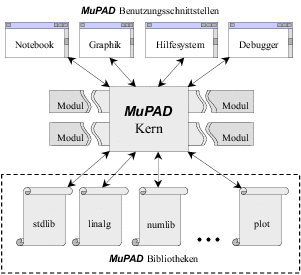
\includegraphics[width=6cm]{figures/figures/components.png}
%\end{center}
%\end{frame}

% \begin{frame}{Kern von Sage ??}
% \begin{itemize}
% \item \alert{Parser:} Liest die Eingaben und überprüft die Syntax;
%   Umwandlung in MuPAD-Datentyp
% \item \alert{Auswerter:} Auswertung und Vereinfachung der
%   Ergebnisse
% \item \alert{Speicherverwaltung:} (MAMMUT $\equiv$ Memory
%   Allocation Managment Unit) interne Verwaltung der
%   MuPAD-Objekte
% \item \alert{Kernfunktionen:}  Oft benötigte Funktionen
%   werden aus Effizienzgründen im Kern auf C-Ebene implementiert.
% \end{itemize}
% \end{frame}

%\begin{frame}{Literatur}
%\begin{itemize}
%\item K. Gehrs, F. Postel. MuPAD -- Eine praktische
%  Einführung. SciFace. 2001.
%\item Ch. Creutzig, J. Gerhard, W. Oevel, St. Wehmeier. Das MuPAD
%  Tutorium. Springer. 2. Auflage. 2002.
%\item M. Majewski. MuPAD Pro Computing Essentials. Springer. 2002.
%\item Rolf Monnerjahn. Mathematische Anwendungen in Biologie, Chemie, Physik. MuPad im Mathematikunterricht: 5.-10. Schuljahr
%\item  Gerd Rapin, Thomas Wassong, Stefan Wiedmann und Stefan Koospal. MuPAD: Eine Einführung
%\end{itemize}
%\end{frame}

%%%%%%%%%%%%%%%%%%%%%%%%%%%%%%%%%%
\section{Streifzug durch Sage}
%%%%%%%%%%%%%%%%%%%%%%%%%%%%%%%%%


\begin{frame}[fragile]{Sage als Taschenrechner}
Hier einige Beispiele: 
\begin{sagecommandline}
sage: 3+4*10+12 
\end{sagecommandline}
\begin{sagecommandline}
sage: sin(pi) 
\end{sagecommandline}
\begin{sagecommandline}
sage: float(pi)
\end{sagecommandline}
\begin{sagecommandline}
sage: float(sqrt(2))
\end{sagecommandline}
\end{frame}



%%%%%%%%%%%%%%%%%%%%%%%%%%%%%%%
%\subsection{Eine Kurvendiskussion}
%%%%%%%%%%%%%%%%%%%%%%%%%%%%%%%%%%
%
%% -> sage.math.uni-goettingen.de
%\begin{frame}[fragile]{Kurvendiskussion I}
%Betrachte die durch die reelle Zahl $a$ parametrisierte Funktionenschar:
%\[ 
%f: x \quad \mapsto \quad \frac{2x^2-20x+42}{x-1}+a, \quad
%a \in \mathbb{R} 
%\]
%
%\begin{itemize}
%\item Eingabe der Funktion
%\begin{sagecommandline}
%sage: a=var('a')
%sage: f(x) = (2*x^2-20*x +42)/(x-1)+a
%\end{sagecommandline}
%\begin{sageout}
%  x |--> a + 2*(x^2 - 10*x + 21)/(x - 1)
%\end{sageout}
%\end{itemize}
%\end{frame}
%
%\begin{frame}[fragile]{Kurvendiskussion II}
%\begin{itemize}
%\item Pol ?
%\begin{sagecommandline}
%sage: f.limit(x=1, dir='minus')
%\end{sagecommandline}
%\begin{sagecommandline}
%sage: f.limit(x=1, dir='plus') 
%\end{sagecommandline}
%%\item Umformen
%%\begin{sagecommandline}
%%f.full_simplify()
%%\end{sagecommandline}
%%\begin{sageout}
%%x |--> ((a - 20)*x + 2*x^2 - a + 42)/(x - 1)
%%\end{sageout}
%\end{itemize}
%\end{frame}
%
%\begin{frame}[fragile]{Kurvendiskussion III}
%\begin{itemize}
%\item Nullstellen
%\begin{sagecommandline}
%sage: solve(f==0,x)
%\end{sagecommandline}
%\begin{scriptsize}
%\end{scriptsize}
%\item Berechnen der Ableitung
%\begin{sagecommandline}
%sage: f.differentiate(x)
%\end{sagecommandline}
%\end{itemize}
%\end{frame}
%
%\begin{frame}[fragile]{Kurvendiskussion IV}
%\begin{itemize}
%\item Extremwerte
%\begin{sagecommandline}
%sage: maxi = solve(f.differentiate(x)==0,x); maxi 
%\end{sagecommandline}
%\begin{sageout}
%[x == -2*sqrt(3) + 1, x == 2*sqrt(3) + 1]
%\end{sageout}
%\item Lokale Minima und Maxima
%\begin{sagecommandline}
%sage: float( ((f.diff(x)).diff(x))(maxi[0].rhs()) )
%\end{sagecommandline}
%\begin{sagecommandline}
%sage: float( ((f.diff(x)).diff(x))(maxi[1].rhs()) )
%\end{sagecommandline}
%\end{itemize}
%\end{frame}
%
%\begin{frame}[fragile]{Kurvendiskussion V}
%\begin{itemize}
%\item Verhalten von $f$ für große $x$
%\begin{sagecommandline}
%sage: f.limit(x=oo); f.limit(x=-oo)
%\end{sagecommandline}
%\begin{sageout}
%x |--> +Infinity
%x |--> -Infinity
%\end{sageout}
%\item Definiere $f_{0}$, $f_{1}$, $f_{2}$
%\begin{sagecommandline}
%sage: f0 = f(x, a=0)
%sage: f1 = f(x, a=-20)
%sage: f2 = f(x, a=20);f0,f1,f2
%\end{sagecommandline}
%\begin{scriptsize}
%\begin{sageout}
%(2*(x^2 - 10*x + 21)/(x - 1), 2*(x^2 - 10*x + 21)/(x - 1) - 20, 2*(x^2 - 10*x + 21)/(x - 1) + 20)
%\end{sageout}
%\end{scriptsize}
%\end{itemize}
%\end{frame}
%
%\begin{frame}[fragile]{Plot}
%\begin{sagecommandline}
%p = plot(f0,detect_poles='show',xmin=0, xmax=10,color='red')
%p += plot(f1,detect_poles='show',xmin=0, xmax=10,color='green')
%p += plot(f2,detect_poles='show',xmin=0, xmax=10,color='blue'); p.show(ymin=-80, ymax=80)
%\end{sagecommandline}
%\begin{center}
%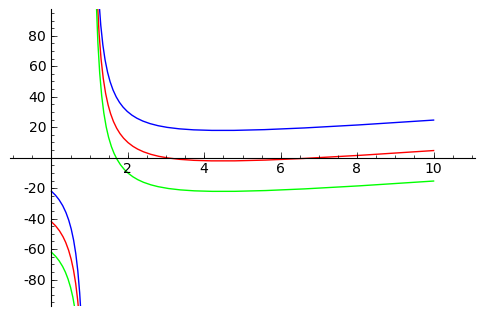
\includegraphics[height=4.5cm]{figures/graphen}
%\end{center}
%\end{frame}

%\begin{frame}[fragile]{Zusammenfassung}
%\begin{itemize}
% \item Deklarieren von Variablen mir \isage{var()}, z.B.{\verb~var('a')~} 
%\item Definieren von Variablen mit {\color{blue}'='}, z.B. {\verb~a=3~} 
%\item Definieren von Funktionen mit{\color{blue} '='}, z.B. {\verb~f(x) = x^2 - 6*x~}
%%\item Symbolisches Rechnen 
%%\begin{itemize}
%\item Grenzwertbestimmung: {\color{blue}   \verb~f.limit(x=1, dir='<plus|minus>')~}
%%\item Vereinfachen: {\color{blue}  \verb~f.full_simplify()~}
%\item Bilden von Ableitungen {\color{blue} \verb~f.differentiate(x)~}
%%\end{itemize} 
%%\end{itemize}
%%\begin{itemize}
%\item Lösen von Gleichungen: {\color{blue} \verb~solve( f(x)==0, x)~}
%\item Berechnen numerischer Approximationen:
%  {\color{blue} \verb~float(f(sqrt(3)+ 4))~}
%\item Plotten einer Funktion: {\color{blue} \verb~plot(sin,(0,4))~}
%\end{itemize}
%\end{frame}

%%%%%%%%%%%%%%%%%%%%%%%%%%%%%%%
%\subsection{Symbolisches Rechnen}
%%%%%%%%%%%%%%%%%%%%%%%%%%%%%%%%%%
%
%\begin{frame}[fragile]{Symbolisches Rechnen I}
%\begin{itemize}
%\item Integrieren von $\int_0^\infty x^4 e^{-x} dx$
%\begin{sagecommandline}
%integrate(x^4*exp(-x),x,0,oo)
%\end{sagecommandline}
%\begin{sageout}
%  24
%\end{sageout}
%\item Stammfunktion von $\frac{1+\sin (x)}{1+\cos(x)}$
%\begin{sagecommandline}
%f(x) = (1+sin(x))/(1+cos(x))
%g = f.integrate(x)
%\end{sagecommandline}
%\begin{sageout}
%x |--> sin(x)/(cos(x) + 1) - log(cos(x) + 1)
%\end{sageout}
%\item Vereinfachen
%\begin{sagecommandline}
%g.full_simplify()
%\end{sagecommandline}
%%\begin{scriptsize}
%\begin{sageout}
%x |--> -((cos(x) + 1)*log(cos(x) + 1) - sin(x))/(cos(x) + 1)
%\end{sageout}
%%\end{scriptsize}
%\end{itemize}
%\end{frame}
%
%\begin{frame}[fragile]{Symbolisches Rechnen II}
%\begin{itemize}
%\item Faktorisieren und Ausmultiplizieren 
%\begin{sagecommandline}
%expand((x-1)*(x-2)*(x-3)*(x-4))
%\end{sagecommandline}
%\begin{sageout}
%x^4 - 10*x^3 + 35*x^2 - 50*x + 24
%\end{sageout}
%\begin{sagecommandline}
%factor(_)
%\end{sagecommandline}
%\begin{sageout}
%(x - 4)*(x - 3)*(x - 2)*(x - 1)
%\end{sageout}
%\item Sortieren eines Ausdrucks bezüglich einer Unbekannten
%\begin{sagecommandline}
%var('b,a')
%g = x^2+2*x+b*x^2+sin(x)+a*x
%g.collect(x)
%\end{sagecommandline}
%\begin{sageout}
%(b + 1)*x^2 + (a + 2)*x + sin(x)
%\end{sageout}
%\end{itemize}
%\end{frame}
%
%\begin{frame}[fragile]{Symbolisches Rechnen III}
%\begin{itemize}
%\item Partialbruchzerlegung
%\begin{sagecommandline}
%g = x^ 2/( x^ 2- 1)
%g.partial_fraction()
%\end{sagecommandline}
%\begin{sageout}
%1/2/(x - 1) - 1/2/(x + 1) + 1
%\end{sageout}
%\item Vereinfachen von Ausdrücken ($\frac{e^x -1}{e^{(1/2)x}+1}$)
%\begin{sagecommandline}
%g = (exp(x)-1)/(exp(x/2)+1)
%g.simplify_radical()
%\end{sagecommandline}
%\begin{sageout}
% e^(1/2*x) - 1
%\end{sageout}
%\end{itemize}
%\end{frame}
%
%\begin{frame}[fragile]{Zusammenfassung}
%\begin{itemize}
%\item symbolisch Integrieren: {\color{blue} \verb~integrate(f,x)~}
% \item numerisch Integrieren: {\color{blue} \verb~integrate(f,x,a,b)~}
%\item faktorisieren: {\color{blue} \verb~expand(f)~}
%\item sortieren: {\color{blue} \verb~f.collect(x)~}
%\item partialbruchzerlegung: {\color{blue} \verb~f.partial_fraction()~}
%\item vollständiges Vereinfachen: {\color{blue} \verb~f.full_simplify()~}
%\item Vereinfachen mit radicals: {\color{blue} \verb~f.radical_simplify()~}
%\end{itemize}
%\end{frame}

% \begin{frame}[fragile]{MuPAD unterscheidet 
% strikt zwischen Funktionen und Ausdrücken I}
% 
% Beispiele:
% 
% \begin{sagecommandline}
% f:= x -> sin(x)
% \end{sagecommandline}
% \begin{sageout}
%  x -> sin(x)
% \end{sageout}
% \begin{sagecommandline}
% g:=sin(x)
% \end{sagecommandline}
% \begin{sageout}
%   sin(x)
% \end{sageout}
% \begin{sagecommandline}
% f(1),g(1)
% \end{sagecommandline}
% \begin{sageout}
%  sin(1), sin(x)(1)
% \end{sageout}
% \end{frame}

% \begin{frame}[fragile]{MuPAD unterscheidet 
% strikt zwischen Funktionen und Ausdrücken II}
% \begin{sagecommandline}
% int(f,x)
% \end{sagecommandline}
% \begin{sageout}
%   Error: Illegal integrand [int]
% \end{sageout}
% \begin{sagecommandline}
% int(f(x),x)
% \end{sagecommandline}
% \begin{sageout}
%   -cos(x)
% \end{sageout}
% \begin{sagecommandline}
% f(x)-g
% \end{sagecommandline}
% \begin{sageout}
%   0
% \end{sageout}
% \begin{sagecommandline}
% h:=fp::unapply(g)
% \end{sagecommandline}
% \begin{sageout}
%   x -> sin(x)
% \end{sageout}
% \end{frame}


%%%%%%%%%%%%%%%%%%%%%%%%%%%%%%%
%\subsection{Etwas AGLA}
%%%%%%%%%%%%%%%%%%%%%%%%%%%%%%%%%%
%
%
%\begin{frame}{Analytische Geometrie und Lineare Algebra}
%
%Berechnen des Schnittpunkts der Ebene 
%\[ E: \vec{x}= 
%\left ( \begin{array}{c}  2 \\ 1 \\ -1 \end{array} \right) +l 
%\left ( \begin{array}{c}  1 \\ -1 \\ -1 \end{array} \right) +m
%\left ( \begin{array}{c}  -3 \\ 1 \\ 4 \end{array} \right), \quad l,m
%\in \mathbb{R}
%\]
%mit der Geraden 
%\[
%g: \vec{x}=
%\left ( \begin{array}{c}  3 \\ 0 \\ 1 \end{array} \right) +k
%\left ( \begin{array}{c}  4 \\ -1 \\ 2 \end{array} \right), \quad k \in \mathbb{R}
%\]
%\end{frame}
%
%\begin{frame}[fragile]{Grafische Darstellung}
%\begin{sagecommandline}
%var('l,m'); E1 = 2+l-3*m; E2 = 1-l+m; E3 =-1-l+4*m
%p = parametric_plot3d([E1,E2,E3],(l,-2,2),(m,-2,2), color='green', opacity=0.8)
%var('k'); g1 = 3+4*k; g2 = -k; g3 = 1+2*k
%p += parametric_plot3d( (g1,g2,g3), (k, -3, 3),thickness='3' ) 
%p.show()
%\end{sagecommandline}
%\end{frame}
%
%\begin{frame}{Grafische Darstellung}
%\begin{center}
%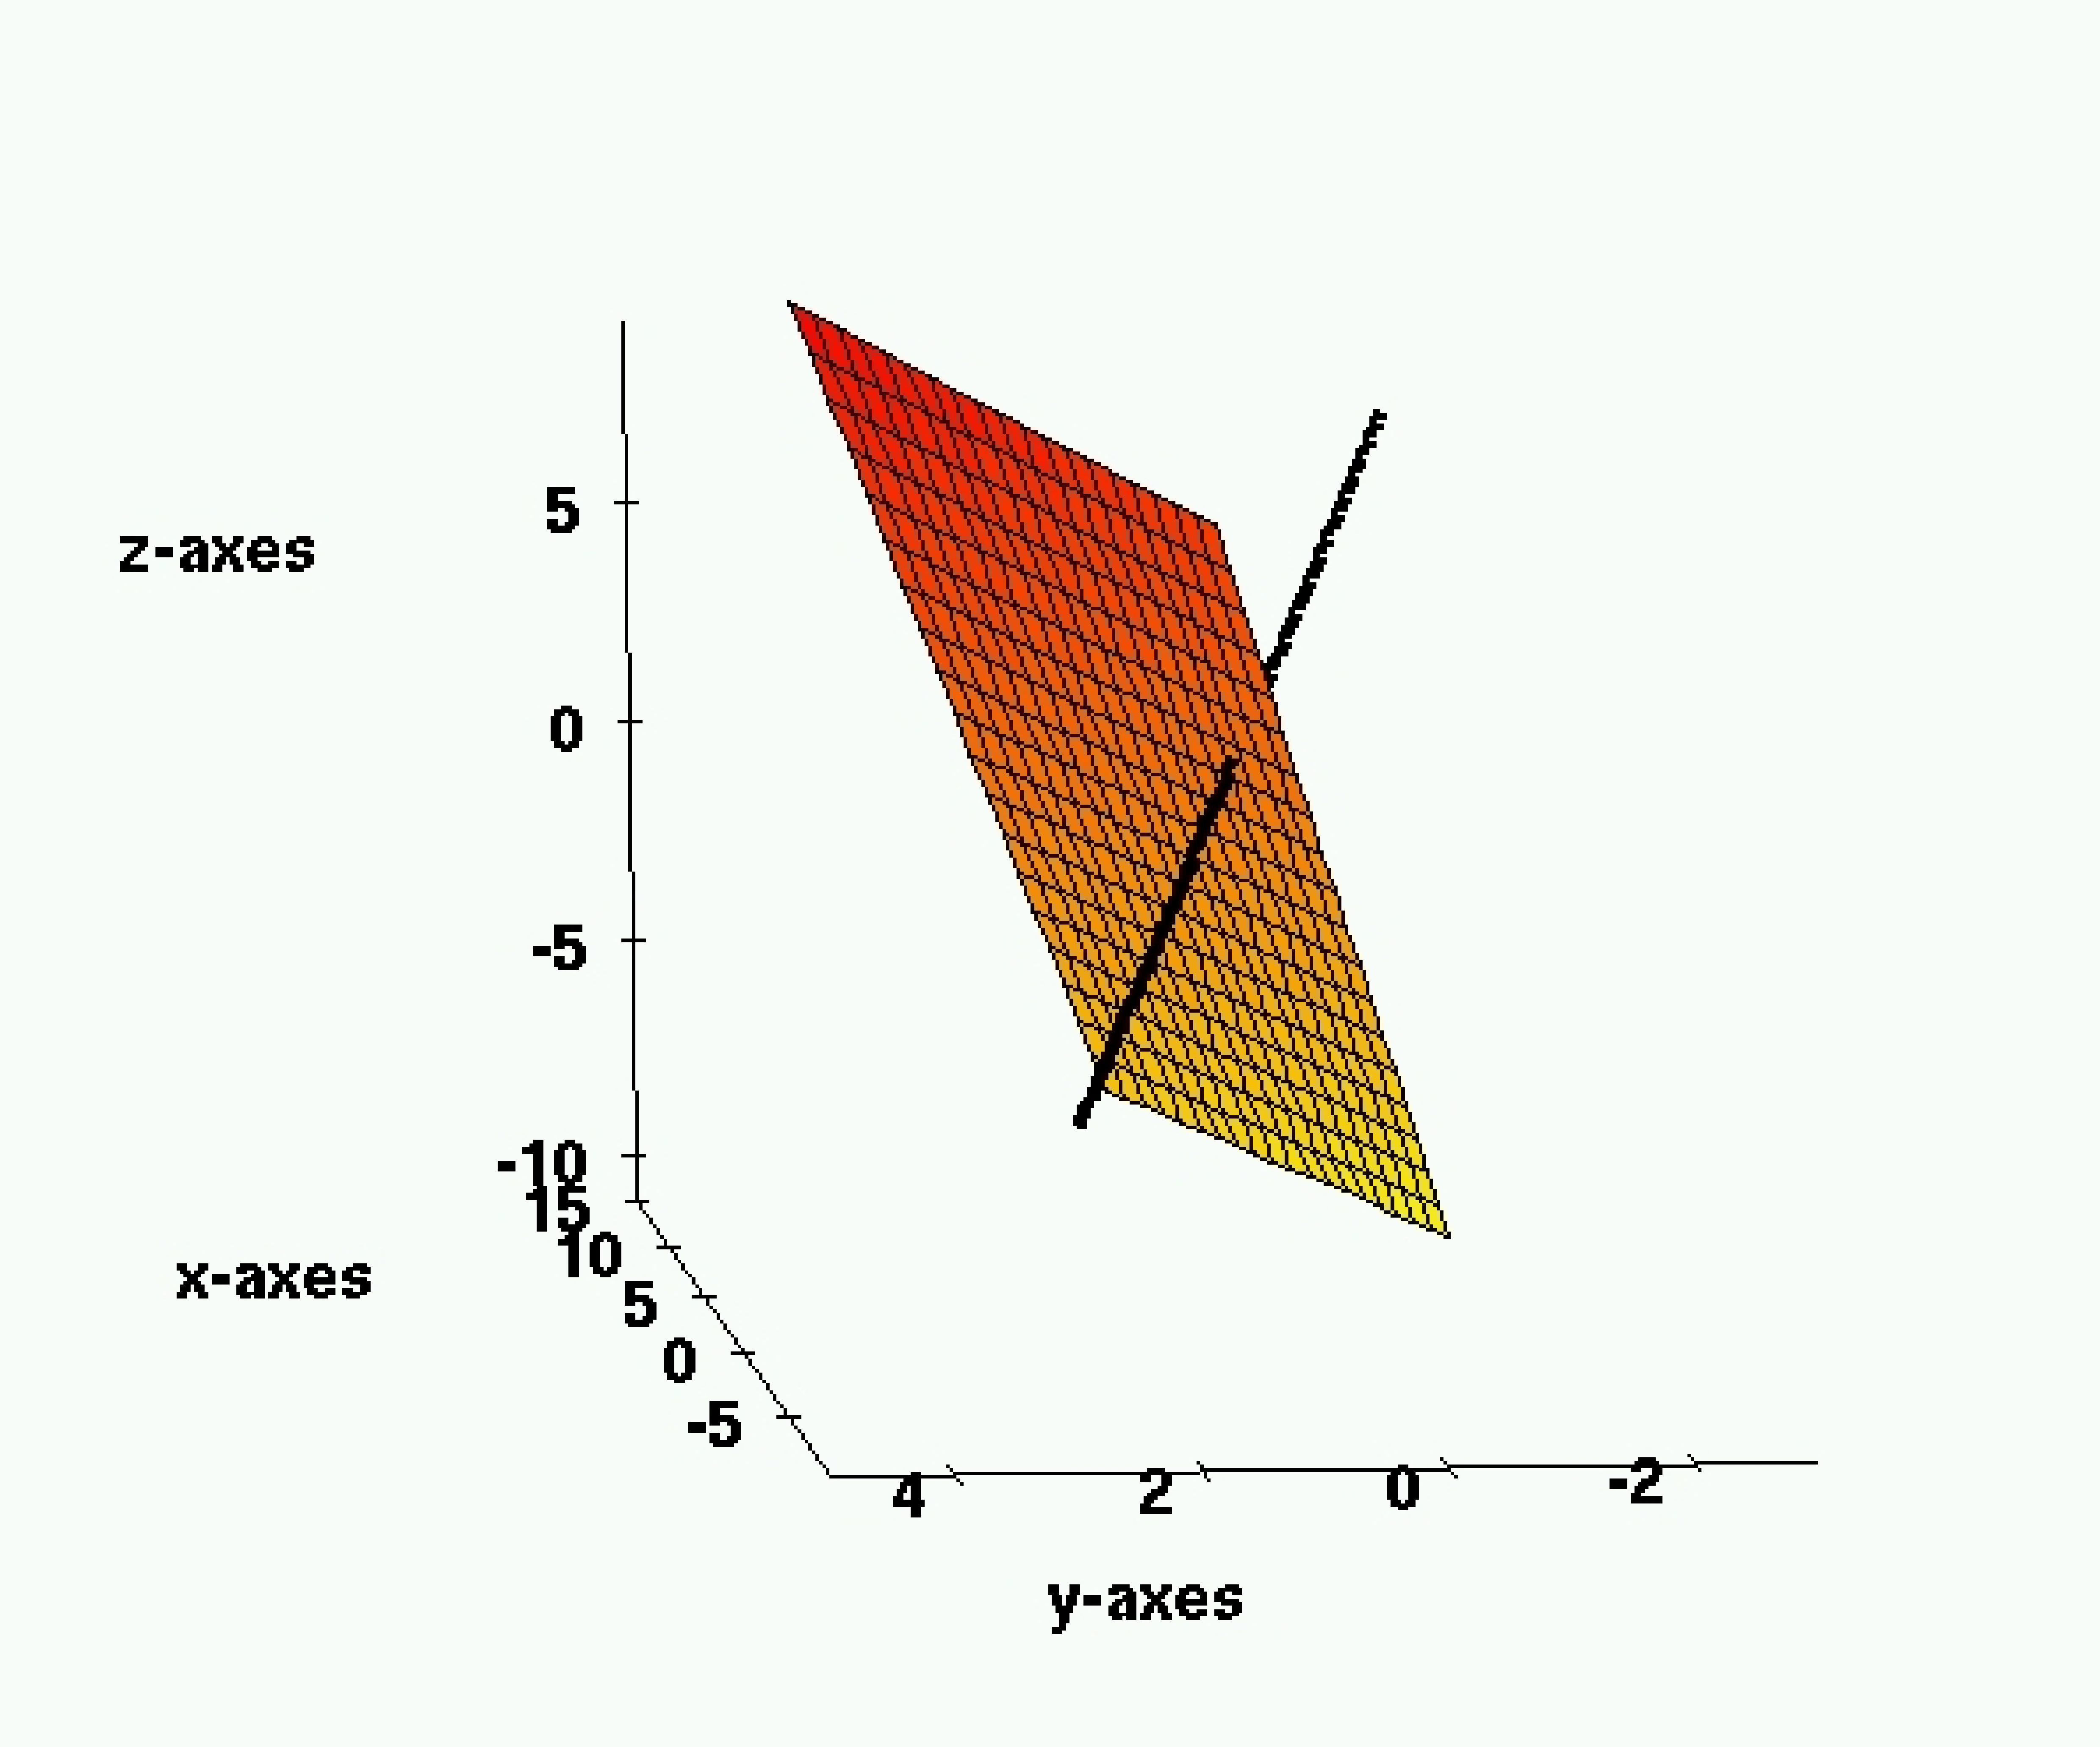
\includegraphics[width=0.7\textwidth]{figures/ebene2}
%\end{center}
%\end{frame}
%
%\begin{frame}{Analytische Lösung}
%Gleichsetzen ergibt: 
%\[ 
%\left ( \begin{array}{c}  2 \\ 1 \\ -1 \end{array} \right) +l 
%\left ( \begin{array}{c}  1 \\ -1 \\ -1 \end{array} \right) +m
%\left ( \begin{array}{c}  -3 \\ 1 \\ 4 \end{array} \right) = \left ( \begin{array}{c}  3 \\ 0 \\ 1 \end{array} \right) +k
%\left ( \begin{array}{c}  4 \\ -1 \\ 2 \end{array} \right)
%\] oder {
%\[ 
%\underbrace{\left(   
%\begin{array} {ccc} 
%1 & -3 & -4\\
%-1 & 1 & 1 \\
%-1 & 4 & -2  
%\end{array} \right)}_{\displaystyle =:A} 
%\underbrace{\left ( \begin{array}{c}  l \\ m \\ k \end{array}
%  \right)}_{\displaystyle =:L} = \underbrace{\left ( \begin{array}{c}  1 \\ -1 \\ 2
%  \end{array} \right)}_{\displaystyle =:b}
%\] }
%oder $A L=b$.
%\end{frame}
%
%\begin{frame}[fragile]{Definieren und Lösen des LGS}
%\begin{itemize}
%\item Definieren der Matrix $A$
%\begin{sagecommandline}
%A = matrix([[1,-3,-4],[-1,1,1],[-1,4,-2]]); A
%\end{sagecommandline}
%\begin{sageout}
%[ 1 -3 -4]
%[-1  1  1]
%[-1  4 -2]
%\end{sageout}
%\item Definieren des Vektors $b$
%\begin{sagecommandline}
%b = vector([1,-1,2])
%\end{sagecommandline}
%\end{itemize}
%\end{frame}
%
%\begin{frame}[fragile]
%\begin{itemize}
%\item Lösen von  $A \ L=b$
%\begin{sagecommandline}
%A.solve_right(b)
%\end{sagecommandline}
%oder 
%\begin{sagecommandline}
%A\b
%\end{sagecommandline}
%ergibt
%\begin{sageout}
%(6/5, 3/5, -2/5)
%\end{sageout}
%\item Einsetzen in die Geradengleichung
%\begin{sagecommandline}
%x_s = matrix([g1,g2,g3]).subs(k=L[2]); x_s
%\end{sagecommandline}
%\begin{sageout}
%[7/5 2/5 1/5]
%\end{sageout}
%\end{itemize}
%\end{frame}
%
%\begin{frame}[fragile]
%\begin{itemize}
%\item Matrizenoperationen
%\begin{sagecommandline}
%B = matrix([[1,0,0],[0,1,1],[1,1,1]])
%A*B; A-B; A+B
%\end{sagecommandline}
%\begin{scriptsize}
%\begin{sageout}
%[-3 -7 -7]  [ 0 -3 -4] [ 2 -3 -4]
%[ 0  2  2]  [-1  0  0] [-1  2  2]
%[-3  2  2]  [-2  3 -3] [ 0  5 -1]
%\end{sageout}
%\end{scriptsize}
%\item Berechnen der Inversen (mit Probe)
%\begin{sagecommandline}
%A^(-1), A*A^(-1)
%\end{sagecommandline}
%\begin{scriptsize}
%\begin{sageout}
%[  -2/5 -22/15   1/15]
%[  -1/5   -2/5    1/5]
%[  -1/5  -1/15  -2/15]
%
%[1 0 0]
%[0 1 0]
%[0 0 1]
%\end{sageout}
%\end{scriptsize}
%\end{itemize}
%\end{frame}
%
%\begin{frame}[fragile]{Zusammenfassung}
%\begin{itemize}
%\item Matrix eingeben: {\color{blue} \verb~matrix([ [z1s1,z1s2],[z2s1,z2s2] ])~}
% \item Vektor eingeben: {\color{blue} \verb~vector([a,b,c])~}
%\item LGS lösen: {\color{blue} \verb~A\b~}
%\item Matrixoperationen: {\color{blue} \verb~A+B,A-B,A*B~}
%\item Matrix invertieren: {\color{blue} \verb~A^(-1); A.inverse()~}
%\item Substitutieren: {\color{blue} \verb~f.subs(k=2)~}
%\end{itemize}
%\end{frame}


%%%%%%%%%%%%%%%%%%%%%%%%%%%%%%%
%\subsection{Etwas Programmieren}
%%%%%%%%%%%%%%%%%%%%%%%%%%%%%%%%%%
%
%\begin{frame}[fragile]{Funktionen}
%\begin{itemize}
% \item eine einzeilige Funktion kann man wie folgt definieren:
%\begin{sagecommandline}
%def <name>(<Argumente>) : return <Rueckgabe>
%\end{sagecommandline}
%\item Beispiel: 
%\begin{sagecommandline}
%def fd(ex) : return diff(ex)
%fd(x^2)
%\end{sagecommandline}
%\begin{sageout}
% 2*x
%\end{sageout}
%\end{itemize}
%\end{frame}
%
%\begin{frame}[fragile]{Listen und Tuple}
% \begin{itemize}
%\item Eine \alert{Liste} ist in Sage (und Python) mit \isage{[..,..]} gekennzeichnet 
%\begin{sagecommandline}
%liste = [21,22,24,23]
%liste.sort(); liste 
%\end{sagecommandline}
%\begin{sageout}
% [21, 22, 23, 24]
%\end{sageout}
%\item Ein \alert{Tuple} ist in Sage (und Python) mit \isage{(..,..)} gekennzeichnet 
%\begin{sagecommandline}
%tuple = (liste[0], liste[2])
%tuple, tuple[0]
%\end{sagecommandline}
%\begin{sageout}
%((21, 24), 21) 
%\end{sageout}
%\item Liste von ganzen Zahlen von \isage{a} bis \isage{b}
%\begin{sagecommandline}
%[a..b] ; range(a,b+1)
%\end{sagecommandline}
% \end{itemize}
%\end{frame}
%
%
%\begin{frame}[fragile]{Einfache Schleifen und Abfragen}
%
%Einzeilige Schleifen
%\begin{sagecommandline}
%[<expr(var)> for <var> in <range|liste>] 
%[<expr(var)> for <var> in <range|liste> if <expr>] 
%\end{sagecommandline}
% \begin{itemize}
%\item Beispiel:
%\begin{sagecommandline}
%[m^2 for m in [1..5] ]
%\end{sagecommandline}
%\begin{sageout}
%[1, 4, 9, 16, 25]
%\end{sageout}
%\item Beispiel mit Abfrage:
%\begin{sagecommandline}
%[m^2 for m in [1..5] if m%2==0]
%\end{sagecommandline}
%\begin{sageout}
% [4, 16]
%\end{sageout}
%
% \end{itemize}
%
% 
%\end{frame}



%%%%%%%%%%%%%%%%%%%%%%%%%%%%%%%
%\subsection{Etwas Zahlentheorie}
%%%%%%%%%%%%%%%%%%%%%%%%%%%%%%%%%%
%
%\begin{frame}[fragile]{Etwas Zahlentheorie I}
%Fermatsche Primzahlen: $F_n=2^{2^n} +1$. Finden Sie die kleinste
%Zahl $F_n$, die keine Primzahl ist!
%\begin{sagecommandline}
%def F(n): return 2^(2^n)+1
%[[F(m),is_prime(F(m))] for m in range(1,6)]
%\end{sagecommandline}
%\begin{sageout}
%[[5, True], [17, True], [257, True], [65537, True], [4294967297, False]]
%\end{sageout}
%\begin{sagecommandline}
%divisors(int(F(5)))
%\end{sagecommandline}
%\begin{sageout}
%[1, 641, 6700417, 4294967297]
%\end{sageout}
%\end{frame}
%
%\begin{frame}[fragile]{Etwas Zahlentheorie II}
%\begin{itemize}
%\item Eine Liste der ersten  Primzahlen bis $100$
%\begin{sagecommandline}
%menge = range(1,101)
%[m for m in menge if is_prime(m)]
%oder filter(is_prime,menge)
%\end{sagecommandline}
%\begin{sageout}
%[2, 3, 5, 7, 11, 13, 17, 19, 23, 29, 31, 37, 41, 43, 47, 53, 59, 61, 67, 71, 73, 79, 83, 89, 97]
%\end{sageout}
%\item Mersenne-Primzahlen $2^p-1$, $p$ Primzahl. Bestimmen der ersten
%Mersenne Primzahlen im Bereich $\leq 200$.
%\begin{sagecommandline}
%menge = range(1,201)
%primes = [m for m in menge if is_prime(m)]
%[2^m-1 for m in primes if is_prime(2^m-1)]
%\end{sagecommandline}
%\begin{sageout}
%[3, 7, 31, 127, 8191, 131071, 524287, 2147483647, 2305843009213693951,
%618970019642690137449562111, 162259276829213363391578010288127,
%170141183460469231731687303715884105727]
%\end{sageout}
%\end{itemize}
%\end{frame}
%
%\begin{frame}[fragile]{Etwas Zahlentheorie III}
%Wir geben für die natürlichen Zahlen $\leq 1000$ an, wieviele Zahlen
%$1,2,3,\dots $ Teiler haben.
%\begin{sagecommandline}
%menge = range(1,1001)
%liste = [number_of_divisors(int(m)) for m in menge]
%[(i,len([m for m in liste if m==i]))for i in range(1,51)]
%\end{sagecommandline}
%
%\begin{sageout}
%[(1, 1), (2, 168), (3, 11), (4, 292), (5, 3), (6, 110), (7, 2), (8,
%180), (9, 8), (10, 22), (11, 0), (12, 97), (13, 0), (14, 5), (15, 4),
%...
%\end{sageout}
%Teiler der Zahl $840$:
%\begin{sagecommandline}
%divisors(840)
%\end{sagecommandline}
%\end{frame}


%%%%%%%%%%%%%%%%%%%%%%%
%\section{Nützliches und Hilfe}
%%%%%%%%%%%%%%%%%%%%%%%%%%%%%%%%
%
%\begin{frame}[fragile]{Überlebensregeln}
%\begin{itemize}
%\item Mehrere Befehle in einer Zeile durch {\color{blue} \isage{;}} trennen. 
%\item Bei Eingaben, die über mehrere Zeilen gehen, kann ein
%  Zeilenumbruch durch {\color{blue} \verb~<ENTER>~} erreicht werden.
%\item Das Auswerten eines Blocks erfolgt mit {\color{blue} \verb~<SHIFT>+<ENTER>~}.
%\item Ein neues Eingabefeld erhält man durch klicken auf den blauen, horizontalen Balken
%\end{itemize}
%\end{frame} 
%
%\begin{frame}{Nützliches}
%\begin{itemize}
%\item {\color{blue} \isage{_} } refenziert die letzte Ausgabe.
%\item Löschen aller eigenen Variablen und Zurücksetzen auf den Anfangsstatus: {\color{blue} \isage{reset()}}
%%\item Anzeigen aller definierten Variablen: {\color{blue} anames(All)}
%%\item Anzeigen aller selbst definierten Variablen: {\color{blue} anames(All,User)}
%\item Das Feld aktivieren von \alert{Typeset} lässt alle Ausgaben von \LaTeX{} rendern.
%%\item profiler und debugger -> commandline
%\item Html- und/oder \LaTeX-Dokumentation:{\color{blue} \verb~<SHIFT>+<KLICK>~ }auf den blauen Balken
%%\item Publish: Im Notebook kann durch klicken des \alert{Publish}-Reiters das Notebook für alle offen gelegt werden. 
%%\item Unter dem Menupunkt \alert{File} kann man 
%\end{itemize}
%\end{frame}
%
%\begin{frame}[fragile]{Hilfefunktionen in Sage}
%
%\begin{itemize}
%\item {\color{blue} Autocompletion :} mit der {\color{blue} \verb~<TAB>~}-Taste erhält man alle möglichen Funktions- und/oder Variablen-Namen im gegebenen Kontext.\\
%Dies gilt insbesondere auch für Objektfunktionen (\isage{object.function()})
%\item {\color{blue} \isage{<command>?} :} gibt ausführliche Hilfe zu \isage{command} an.
%\item {\color{blue} \isage{help(<command>)} :} öffnet ein Hilfefenster zu \isage{command}.
%\item online Dokumentation: 
%\begin{itemize}
%\item Sage: \url{http://www.sagemath.org/doc/index.html}
%\item Python: \url{http://docs.python.org/}
%\end{itemize}
%\end{itemize}
%\end{frame}
\end{document}
